\documentclass{beamer}
\usetheme{metropolis}

\usepackage{enumitem}
\setlist[itemize,1]{before*=\normalsize,label=$\bullet$}
\setlist[itemize,2]{before*=\small,label=$\circ$}
\setlist[itemize,3]{before*=\footnotesize,label=\Smiley}

\usepackage{marvosym}
\usepackage{tikz}

\title{%
  Discrete Channels w/Noise \\
  \normalsize A Mathematical Theory of Communication, Part II}
\author{David Sanders}

\begin{document}

  \maketitle

  \section{First, some review... \small (p.1 -- 19)}

  \begin{frame}{Introduction}
    \begin{columns}

      \column{\dimexpr\paperwidth-10pt}

      \begin{itemize}
        \item Context of signal processing (PCM, PPM)
        \item Communication is about reproducing messages sent over channels
        \item Mathematical theory shouldn't care about meaning of messages
        \begin{itemize}
          \item Instead, focus is on message as one selected from many possible
          \item Absence of meaning allows messages to be viewed as random variables
        \end{itemize}
        \item Any monotonic increasing function of number of possible messages
        is measure of information
        \begin{itemize}
          \item Logarithm is best choice
          \begin{itemize}
            \item Engineering parameters vary linearly w/log of possibilities
            \item More intuitive -- 2 disks have twice the information ($(2^x)(2^x) = 2^{2x}$ states)
            \item Mathematically convenient -- ``downgrades" operations; $\log ab = \log a + \log b$, etc.
          \end{itemize}
        \end{itemize}
      \end{itemize}

    \end{columns}
  \end{frame}

  \section{Discrete Noisy Channels \small (p.19 -- 28)}

  \begin{frame}{Basic Concepts}
    What is noise?
    \begin{itemize}
      \item Perturbation of transmitted signal ($S$) by noise ($N$) at either terminal or in channel
      \item Received signal ($E$) may not be same as transmitted signal ($S$)
    \end{itemize}

    \begin{figure}
      \footnotesize
      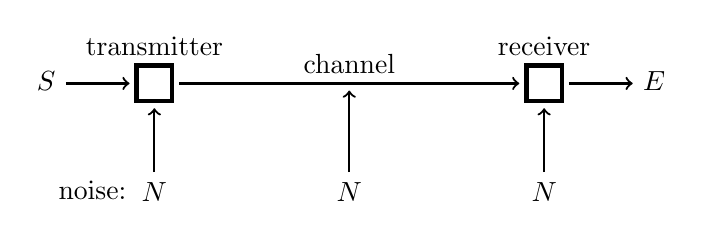
\begin{tikzpicture}[scale=0.45,->,thick]
        \draw (-2,0.5) -- (-0.2,0.5);
        \node [left] at (-2,0.575) {$S$};
        \node [below left] at (0,-1.95) {noise:};

        \draw (0.5,-2) -- (0.5,-0.2);
        \node [below] at (0.5,-2) {$N$};

        \draw [ultra thick] (0,0) rectangle (1,1);
        \node [above] at (0.5,1) {transmitter};

        \draw (1.2,0.5) -- (10.8,0.5);
        \node [above] at (6,0.5) {channel};

        \draw (6,-2) -- (6,0.3);
        \node [below] at (6,-2) {$N$};

        \draw [ultra thick] (11,0) rectangle (12,1);
        \node [above] at (11.5,1) {receiver};

        \draw (11.5,-2) -- (11.5,-0.2);
        \node [below] at (11.5,-2) {$N$};

        \draw (12.2,0.5) -- (14,0.5);
        \node [right] at (14,0.575) {$E$};
      \end{tikzpicture}
      \caption{Sources of noise.}
    \end{figure}
  \end{frame}

  \begin{frame}{Kinds of Noise}
    Two different kinds of noise:
    \begin{itemize}
      \item Distortion: $E \neq S$ and $E = f(S)$
      \begin{itemize}
        \item If $f^{-1}$ exists for $f$, recovery of $S$ from $E$ is possible
      \end{itemize}
      \item Random noise: $E \neq S$ and $E = f(S, N)$
      \begin{itemize}
        \item Noise $N$ is random variable; may be represented by stochastic
        process
      \end{itemize}
    \end{itemize}
  \end{frame}

\end{document}
